\footnotesize
\newcommand{\BaseStruct}{
\draw[line width=1.2mm](0,0)|-(3,3);
\node[draw,inner sep=0,minimum size=2.5mm,circle,fill=white,line width=.6mm]at(0,0){};
\node[draw,inner sep=0,minimum size=2.5mm,circle,fill=white,line width=.6mm]at(3,3){};
}
\newcommand{\BaseStructX}{
\draw[line width=1.2mm](0,0)|-(3,3);
\node[draw,inner sep=0,minimum size=2.5mm,circle,fill=white,line width=.6mm]at(0,0){};
}
\newcommand{\BaseStructS}{
\draw[line width=1.2mm](0,0)|-(3,3)--(3,0);
\node[draw,inner sep=0,minimum size=2.5mm,circle,fill=white,line width=.6mm]at(0,0){};
\node[draw,inner sep=0,minimum size=2.5mm,circle,fill=white,line width=.6mm]at(3,0){};
}
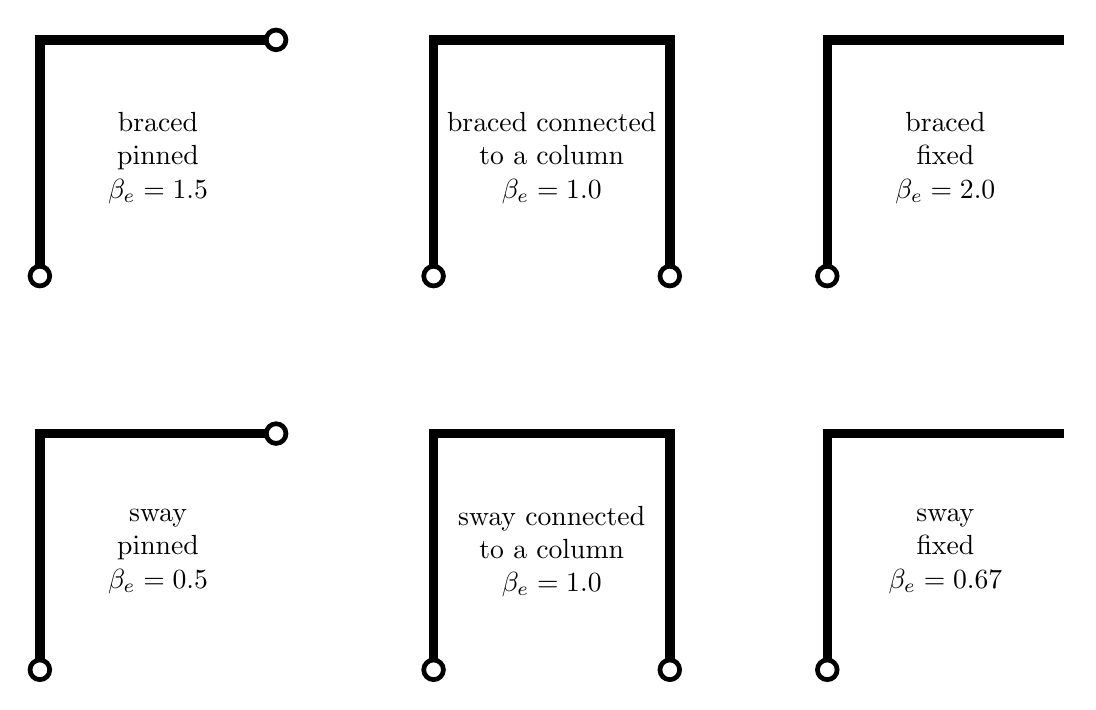
\begin{tikzpicture}
\begin{scope}
\HingeSupport{0,0}
\HingeSupport[90]{3,3}
\BaseStruct
\node[align=center]at(1.5,1.5){braced\\pinned\\$\beta_e=1.5$};
\end{scope}
\begin{scope}[xshift=5cm]
\HingeSupport{0,0}
\HingeSupport{3,0}
\RollerSupport[90]{3,3}
\BaseStructS
\node[align=center]at(1.5,1.5){braced connected\\to a column\\$\beta_e=1.0$};
\end{scope}
\begin{scope}[xshift=10cm]
\HingeSupport{0,0}
\FixedSupport[90]{3,3}
\BaseStructX
\node[align=center]at(1.5,1.5){braced\\fixed\\$\beta_e=2.0$};
\end{scope}
\begin{scope}[yshift=-5cm]
\HingeSupport{0,0}
\RollerSupport{3,3}
\BaseStruct
\node[align=center]at(1.5,1.5){sway\\pinned\\$\beta_e=0.5$};
\end{scope}
\begin{scope}[xshift=5cm,yshift=-5cm]
\HingeSupport{0,0}
\HingeSupport{3,0}
\BaseStructS
\node[align=center]at(1.5,1.5){sway connected\\to a column\\$\beta_e=1.0$};
\end{scope}
\begin{scope}[xshift=10cm,yshift=-5cm]
\HingeSupport{0,0}
\SleeveSupport[90]{3,3}
\BaseStructX
\node[align=center]at(1.5,1.5){sway\\fixed\\$\beta_e=0.67$};
\end{scope}
\end{tikzpicture}